\documentclass{standalone}

\usepackage{tikz}
\usepackage{tikz-3dplot}

\newcommand{\wave}[1] { cos(deg(pi*#1-1)) }

\begin{document}

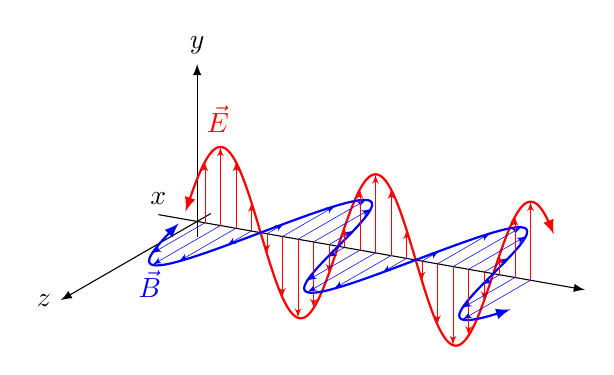
\begin{tikzpicture}[x={(-10:1cm)}, y={(90:1cm)},z={(210:1cm)}]

	% Axes
	\draw[-latex] (-.5, 0, 0) node[above] {$x$} -- (5, 0, 0);
	\draw[-latex] (0, -.2, 0) -- (0, 2, 0) node[above] {$y$};
	\draw[-latex] (0, 0, -.2) -- (0, 0, 2) node[left] {$z$};

	% Waves
	\draw[latex-latex,thick,red]  plot[domain=-.15:4.6, samples=20 0] (\x, {\wave\x}, 0);
	\draw[latex-latex,thick,blue] plot[domain=-.15:4.6, samples=20 0] (\x, 0, {\wave\x});

	% Arrows
	\foreach \x in {0.1,0.3,...,4.3} {
		\draw[-latex',help lines,red]  (\x, 0, 0) -- (\x, {\wave\x}, 0);
		\draw[-latex',help lines,blue] (\x, 0, 0) -- (\x, 0, {\wave\x});
	}

	\node[above right,red] at (0,1,0) {$\vec{E}$};
	\node[below right,blue] at (0,0,1) {$\vec{B}$};

\end{tikzpicture}

\end{document}

